\chapter{Piattaforma numerica \label{cap4}}

 %%%%%%%%%%%%%%%%%%%%%%%%%%%%%%%%%%%%%%%%%%%
\Figure[width=0.98\textwidth]{./figure/platform/flowchart.png}{Schema a 
blocchi descrittivo dei codici all'interno della piattaforma.}{flowchart}
 %%%%%%%%%%%%%%%%%%%%%%%%%%%%%%%%%%%%%%
In questo capitolo sarà descritta la piattaforma numerica che permette 
l'integrazione dei codici di neutronica con i codici termo-idraulici.
I codici di neutronica appartengono alla \textit{Version5}, sviluppata presso 
\'Ecole 
Polytechnique de Montréal e disponibile gratuitamente sul 
\href{https://www.polymtl.ca/merlin/version5.htm}{sito}; si dividono 
principalmente in un 
codice di calcolo di cella/reticolo \textit{Dragon} e in uno di calcolo globale 
di 
reattore.
Il primo si pone lo scopo della creazione di un database reattoristico, il 
quale 
permetterà la successiva interpolazione e costruzione delle sezione d'urto 
macroscopiche omogeneizzate per il corretto funzionamento del codice 
di reattore.
Il codice di reattore, invece, risolve l'equazione del trasporto per ottenere 
il 
flusso neutronico e di conseguenza la potenza termica prodotta dalle reazioni di
fissione degli isotopi fissili e dai processi di decadimento degli isotopi
radioattivi nelle regioni del reattore occupate dagli elementi di 
combustibile.
Vi è la possibilità di effettuare valutazioni con le barre di sicurezza e di 
controllo inserite o estratte, al fine di controllare l'evoluzione della 
popolazione neutronica attraverso inserzioni di reattività. 

%%%%%%%%%%%%%%%%%%%%%%%%%%%%%%%%%%%%%%%%%%%%%%%%%%%%%%%%%%%%%%%%%%%%%%%%%%%
\Figure[width=0.98\textwidth]{./figure/flowchart/dataflow_platform}{Schema a blocchi 
concettuale dell'approccio multifisico.}{platformnumeric}
%%%%%%%%%%%%%%%%%%%%%%%%%%%%%%%%%%%%%%%%%%%%%%%%%%
Il codice di termo-idraulica, attraverso lo scambio di dati relativo alla 
potenza 
termica rilasciata dalle barre di combustibile, risolve le equazioni della 
termodinamica restituendo così il campo di temperatura sull'intero volume del 
reattore.
In questo modo, il campo di temperatura andrà a correggere i valori delle 
sezioni d'urto macroscopiche attraverso l'interpolazione sui parametri contenuti 
nel database 
reattoristico, e creando così un ciclo iterativo dove il codice neutronico scambia 
informazioni con quello termo-idraulico e viceversa.
Una delle caratteristiche della distribuzione \textit{Version5} è la capacità 
di 
essere integrata con la piattaforma \textit{Salom\'e}, attraverso un linguaggio 
di 
scrittura, chiamato \textit{CLE-2000}, che gestisce il flusso di informazioni 
computazionali \cite{DDhebe}.
Lo scopo della piattaforma è di permettere l'accoppiamento dei due codici, 
creando un ambiente semplificato che consente l'interazione tra di essi. 
L'originalità di un approccio multi-fisico è che le diverse componenti software 
sono in grado di cooperare dinamicamente per l'ottimizzazione e la gestione 
delle risorse computazionali.
La piattaforma numerica deriva da un lavoro di modifica di un'altra già 
esistente, la piattaforma NURESAFE, sviluppata dalla CEA per accoppiare codici 
differenti in uno studio di un nuovo progetto di reattori ad acqua leggera.
Il progetto collaborativo NURESAFE per lo sviluppo di programmi affidabili e
utilizzabili per l'analisi di sicurezza di reattori nucleari è stata fondata 
dalla comunità europea basandosi sulla piattaforma open-source 
\textit{Salom\'e}.
Risulta opportuno specificare che tutti i codici presenti sono open-source, ovvero di libera licenza, ma è 
possibile integrare altri codici anche proprietari grazie alle versatilità della 
piattaforma. 

Nelle Figure \ref{flowchart} e \ref{platformnumeric} sono rappresentati gli 
schemi a blocchi che descrivono il comportamento dei codici che garantiscono 
l'accoppiamento neutronico e termoidraulico in riferimento a sistemi nucleari. 


\section{Piattaforma \textit{Salom\'e}}

La piattaforma \textit{Salom\'e} possiede un numero di moduli ciascuno con una 
specifica funzione all'interno della piattaforma stessa. I moduli pi\`u
usati sono i moduli KERNEL, GUI, GEOM, SMESH,
ParaVis, MED e YACS.
Il modulo KERNEL fornisce una struttura comune per tutti gli altri 
componenti, i 
quali possono essere integrati nella piattaforma. Infatti l'architettura di 
\textit{Salom\'e} è basata su un concetto multilayer client/server che rende la piattaforma molto 
flessibile.
Il modulo GUI offre un'interfaccia grafica per l'utilizzo della 
piattaforma.
Molto importante è il modulo GEOM il quale facilita la costruzione e 
l'ottimizzazione dei modelli geometrici, usando un ampia scelta di funzioni CAD.
Il modulo SMESH invece genera le griglie numeriche (mesh) sui modelli 
geometrici 
precedentemente creati o importati dalla componente GEOM. Infatti il 
modulo è in 
grado di creare e di modificare la mesh, importare ed esportarle in 
diversi formati, di creare gruppi di elementi all'interno della mesh, di 
filtrare nodi o elementi della mesh, e di ottenere informazione su di esse e 
sui 
suoi sotto-oggetti per il controllo della qualità.
Il modulo ParaVis consiste nell'integrazione di \textit{ParaView} 
all'interno di \textit{Salom\'e} ed 
ottimizza la visualizzazione dei dati ottenuti attraverso un interfaccia 
grafica. 
Sopra a tutti gli strumenti computazionali inclusi nella piattaforma, il modulo 
MED fornisce le librerie per immagazzinare e recuperare i dati in 
formato MED, 
associando le mesh con i campi numerici e permettendone lo scambio tra i 
differenti codici e risolutori. All'interno di \textit{Salom\'e} le 
strutture di dati vengono 
scambiate tra i risolutori offrendo funzioni comuni di lettura e scrittura 
attraverso i file MED.
Il modulo YACS è uno strumento che supervisiona l'esecuzione 
di applicazioni 
scientifiche complesse e interconnesse su rete di computer e clusters \cite{yacss}. In 
YACS 
queste applicazioni sono descritte da una uno schema di calcolo che può essere 
definito con una sintassi XML e sono principalmente un grafico di nodi che 
riferiscono a obiettivi computazionali e a strutture di controllo. 

%%%%%%%%%%%%%%%%%%%%%%%%%%%%%%%%%%%%%%%%%%%%%%%%%%%%%%%%%%%%5
\Figure[width=0.8\textwidth]{./figure/platform/mappa.png}{Mappatura di ogni nodo di un 
generico elemento nel suo duplicato MED}{mappa}
%%%%%%%%%%%%%%%%%%%%%%%%%%%%%%%%%%%%%%%%%%%%%%%%%%%%%%%%%%%%%%%%
La piattaforma numerica è stato concepita non solamente per raggruppare una 
serie di codici che sono usati in un ambito termo-idraulico di reattori 
nucleari, 
ma anche per armonizzarli con lo scopo di risolvere problemi complessi 
attraverso lo scambio di informazioni tra i differenti codici sopra una 
piattaforma comune \cite{ribes2007salome}.
\textit{Salom\'e} può essere anche usata come una piattaforma per l'integrazione 
di codici 
numerici esterni di terze parti.
L'integrazione del codice sulla piattaforma \textit{Salom\'e} è ottenuto dalla 
generazione 
di un interfaccia con funzioni disponibili nella libreria \textit{MEDMem} che 
consente il 
trasferimento dei dati dalla piattaforma al codice e viceversa.


L'integrazione di un codice open-source in una piattaforma numerica può essere 
suddivisa in tre aspetti principali. Il primo consiste nella generazione di una 
libreria relativa al codice originale, il secondo consiste nella generazione 
dell'interfaccia \textit{MEDMem} e il terzo nella generazione del codice di 
interfaccia 
\textit{Salom\'e}.
Una simulazione richiede la manipolazione di mesh e campi, incluso 
l'accoppiamento di codice per l'elaborazione dei dati o dei risultati. Una 
volta 
costruito il codice come una libreria è necessario aggiungere metodi per 
esportare i risultati in formato MED in modo da passare il campo computazione ad 
un altro codice. Infatti è possibile estrarre la soluzione da un file MED e 
proiettarla in domini computazionali differenti sempre all'interno di file MED. 
A questo fine si crea un duplicato della griglia computazionale originale nel 
file MED e una mappa che associa a ciascun nodo computazionale uno nel suo 
duplicato e viceversa come mostrato in Figura \ref{mappa}.
La mappa così generata permette di trasferire il campo computazionale ad un 
altro mesh MED del dominio di un altro codice computazionale.
Attraverso la mappa e l'interfaccia si consente l'integrazione dei differenti 
codici. Infatti i dati e campi computazionali sono passati tra una MED e 
l'altra 
con lo scopo di consentire la soluzione del problema attraverso uno scambio di dati iterativo.

\begin{figure}[htb!]
\centering
\subfigure[Modello neutronico]
{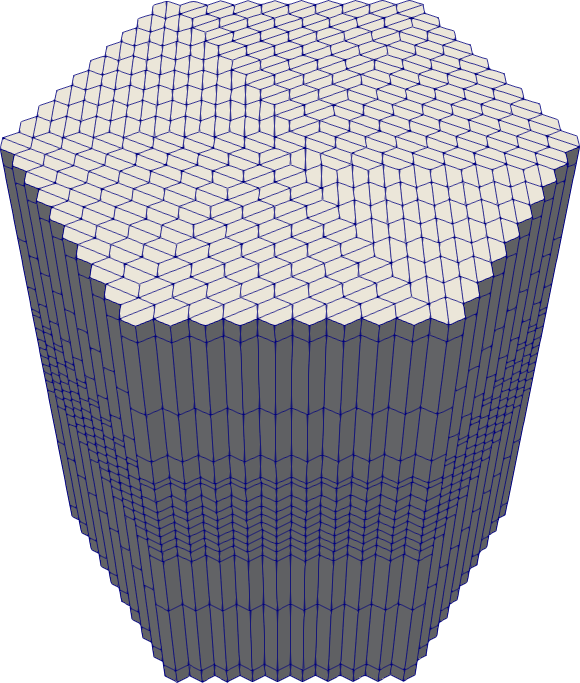
\includegraphics[width=0.48\textwidth]{./figure/result_tred/new/meshneut.png}}\\
% \hspace{5mm}
\subfigure[Modello termodinamico]
{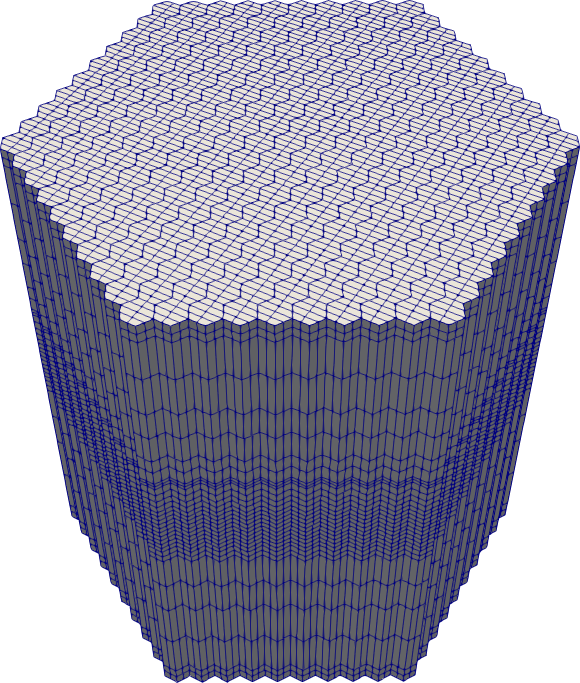
\includegraphics[width=0.48\textwidth]{./figure/result_tred/new/meshtemp.png}}
\caption{Mesh tridimensionale del modello di ALFRED per la neutronica (a) e per la termoidraulica (b).}
\end{figure}



\section{Codice di cella Dragon}
Il codice di cella/reticolo \textit{Dragon} è utilizzato per risolvere 
l'equazione del 
trasporto neutronico attraverso un approccio deterministico sopra un dominio 
corrispondente a una sotto parte o all'intero reattore nucleare considerato.
Infatti è la principale componente software per descrivere il comportamento dei 
neutroni in un reattore nucleare, dove i più importanti fenomeni nucleari sono 
descritti con accuratezza e precisione.
Pertanto il codice \textit{Dragon} include effetti dovuti a variazioni di 
temperatura e densità dei 
materiali, risonanze di auto schermaggio, bruciamento del combustibile, 
trasporto 
e fughe di neutroni. 
Tipicamente il codice di cella è applicato sopra un dominio spaziale denominata 
cella unitaria, la quale rappresenta una regione 2D del reattore che si ripete 
per simmetria o traslazione.
Durante questa tesi, il codice di cella è stato utilizzato per produrre un 
database reattoristico contente il comportamento neutronico applicato alle 
principali strutture che compongono il reattore.
In particolare, è stata creata una struttura dati, denominata 
\texttt{MULTICOMPO}, che 
contiene le proprietà nucleari delle sezioni d'urto macroscopiche degli 
elementi 
di combustibile e degli elementi strutturali, in riferimento a diversi 
parametri 
come la temperatura del combustibile, la temperatura e densità del refrigerante 
e i tempi di bruciamento del combustibile. 

\subsection{Database reattoristico \label{datareactor}}
%\label{datareactor}

% \begin{figure}
% \centering
% \subfigure[Complessivo di un'assemblea]
% {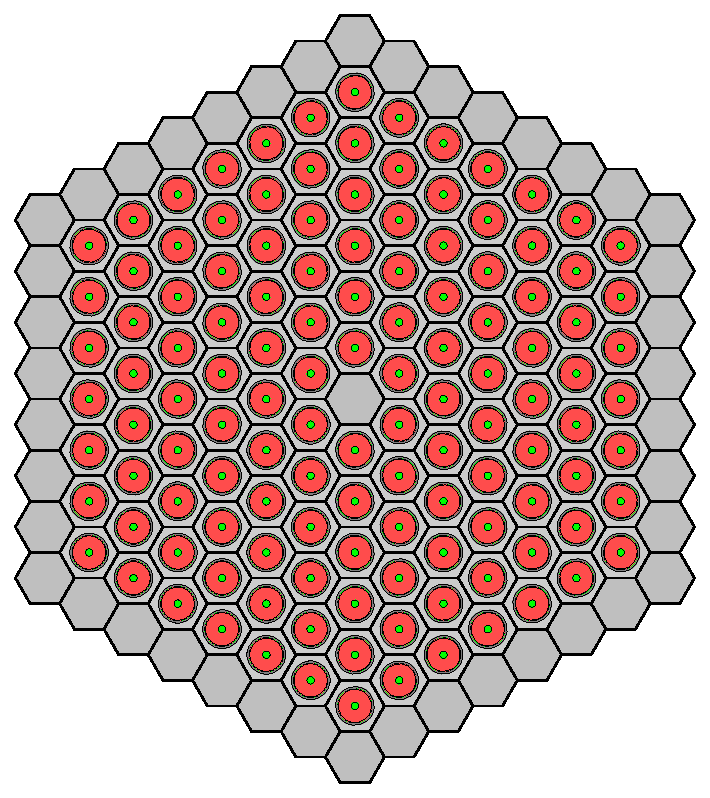
\includegraphics[width=0.45\textwidth]{./figure/itex/fassembly.pdf}}
% % \hspace{5mm}
% \subfigure[Singola cella]
% {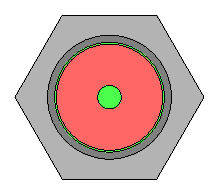
\includegraphics[width=0.3\textwidth]{./figure/itex/unitcells.pdf}}
% \caption{Modellazione dell'assembly (a) e della singola cella (b).}
% \end{figure}
% %%%%%%%%%%%%%%%%%%%%%%%%%%%%%%%%%%%%%%%%%%%%%%%%%%%%%%%%%%%%%%%%%%%%%
Una componente all'interno dei codici di reticolo o di cella è dedicato alla 
costruzione di un database reattoristico con lo scopo di salvare tutti i dati 
nucleari prodotti dal codice, che è indispensabile per la successiva 
implementazione nei calcoli di reattori.
Infatti, dal punto di vista computazionale i calcoli multigruppo di reticolo 
risultano troppo costosi per essere eseguiti dinamicamente all'interno dei 
calcoli di reattore.
Un approccio più flessibile è creare un database reattoristico dove sono 
tabulati un numero finito di calcoli di reticolo in corrispondenza di parametri 
locali o globali, scelti al fine di rappresentare le condizioni operative del 
reattore.
Alcuni parametri locali o globali sono tipicamente il bruciamento, la 
temperatura del combustibile, la temperatura e densità del refrigerante e
l'eventuale concentrazione di boro.
Una volta che il database reattoristico è stato costruito, i moduli relativi al 
calcolo globale di reattore devono ottimizzare l'interpolazione sui valori 
contenuti in esso come una funzione di condizioni locali in ogni mesh del 
dominio del reattore.
Il codice computazionale opera con moduli (MODULE), che assolvono i 
diversi compiti, interagendo tra di loro con strutture oggetto (LINKED LIST), i quali contengono i dati necessari per l'elaborazione dei calcoli.
Inoltre è possibile definire anche dei sotto codici per semplificare la 
leggibilità 
del codice (PROCEDURE).

Successivamente dovranno essere definiti i vettori, contenenti i valori 
associati al tempo di bruciamento, alla temperatura del combustibile, della 
guaina di rivestimento e del refrigerante che sono richiesti dall'utente al fine 
di costruire un 
database in base alle esigenze del problema.
In particolare al tempo di bruciamento, espresso in giorni, è associato anche 
il 
valore di potenza termica aspettata da una assembly di combustibile al fine di 
poter identificare la corretta evoluzione degli isotopi presenti.
Inoltre sono state create delle procedure per rendere il codice più compatto e 
facilmente leggibile; tali procedure contengono, per esempio, il calcolo della 
dilatazione termica e della densità dei materiali a seguito di una variazione di 
temperatura. 
Infatti ad una variazione di temperatura dei materiali è associata una variazione 
di densità dei nuclei; questo effetto influisce sulle sezioni d'urto 
microscopiche.

Al fine di costruire un database reattoristico, è possibile usare diverse 
combinazioni dei moduli che variano in base alle esigenze e anche 
all'accuratezza fisica del problema o in base al costo computazionale.
Concettualmente il primo passo per la costruzione delle sezioni d'urto 
macroscopiche delle componenti del reattore è la definizione della 
geometria dell'assembly e della composizione dei materiali.
I dati nucleari dei materiali sono contenuti all'interno di librerie sulle sezioni 
d'urto microscopiche, le quali saranno caricate all'interno di strutture 
oggetto 
ed elaborate dal codice.
Successivamente viene analizzato il comportamento neutronico, attraverso un 
processo di "\textit{tracking}" della geometria che permette l'analisi con l'aiuto di 
tecniche di risoluzione del 
trasporto neutronico, come il metodo della probabilità di collisione e/o il 
metodo 
delle caratteristiche, descritti nelle Sezioni \ref{metcaratt} e \ref{probcoll}.

Nello specifico sono effettuati dei cicli iterativi per la costruzione del 
database reattoristico. 
In particolare un primo ciclo iterativo è effettuato con lo scopo di ottenere 
le 
sezioni d'urto relative ai tempi di bruciamento di riferimento, con 
l'evoluzione degli 
isotopi nel tempo attraverso un parametro di potenza termica ipotizzata per 
l'assembly di combustibile. 
Questo bruciamento di riferimento è necessario nel secondo ciclo iterativo dove 
invece si analizzano le variazioni di temperatura e di densità dei materiali 
che 
compongono l'assembly.
Alla fine del procedimento si ottengono le sezioni d'urto omogeneizzate 
spazialmente e condensate sulle energie. 

\subsection{Descrizione del procedimento utilizzato}

Al fine di modellare le assembly delle componenti del reattore complessivo, 
sono stati realizzati tre codici differenti.
I primi due codici sono relativi alle assembly di 
combustibile interne e esterne al nocciolo, le quali differiscono solamente per l'arricchimento del 
combustibile ad ossidi misti. Mentre il terzo codice è relativo alle assembly degli elementi strutturali e dei dispositivi, come per esempio le barre di controllo e di sicurezza, i riflettori neutronici ed i elementi di 
protezione neutronica.

Le assembly di combustibile di ALFRED sono state modellate con una geometria 
esagonale composta, a sua volta, da esagoni che rappresentano il singolo elemento 
come la barra di combustibile o l'elemento di contenimento.
%%%%%%%%%%%%%%%%%%%%%%%%%%%%%%%%%%%%%%%%%%%%%%%%%%%%%%
\Figure[width=0.8\textwidth]{./figure/platform/crosection.pdf}{Costruzione 
dell'assembly 
di combustibile attraverso il modulo GEO:.}{crosection}
%%%%%%%%%%%%%%%%%%%%%%%%%%%%%%%%%%%%%%%%%%%%%%%%%%%%%%%%%%%%%%%%%%%%%%%%%%%
In Figura \ref{crosection} è mostrato il modello dell'assembly di combustibile, 
composto dalla cella C1 che rappresenta la singola barra di combustibile mentre 
la cella C2 il materiale di acciaio che contiene e sostiene le barre di 
combustibile.
In particolare la cella C1 rappresenta la singola barra di combustibile ed è 
stata modellata come in figura \ref{pins}, in cui viene specificata il raggio 
delle regioni contenute dal quello più interno a quello più esterno: gas di 
fissione, il combustibile MOX, il gap di elio, la guaina di rivestimento e 
piombo.
%%%%%%%%%%%%%%%%%%%%%%%%%%%%%%%%%%%%%%%%%%%%%%%%%%%%%%
\Figure[width=0.5\textwidth]{./figure/platform/pin.pdf}{Rappresentazione della cella di 
combustibile C1 della geometria in \ref{crosection}.}{pins}
%%%%%%%%%%%%%%%%%%%%%%%%%%%%%%%%%%%%%%%%%%%%%%%%%%%%%%
La cella C2 invece è stata modellata come un esagono di solo acciaio e 
definisce 
l'elemento strutturale e di contenimento della assembly di combustibile.
I valori sulle sezioni d'urto microscopiche dei materiali sono estratti 
dalle librerie dei dati nucleari, quali le librerie JEFF o ENDF/B in base alle 
richieste dell'utente, scaricabili dal 
\href{https://www.polymtl.ca/merlin/libraries.htm}{sito};
% In questo caso saranno utilizzate la versione 3.1.2 delle JEFF a 315 gruppi, 
è possibile sostituirle facilmente attraverso la modifica dello script di 
accesso alle librerie.
Viene così assemblata la geometria dell'assembly comprendente della composizione 
dei materiali 
ed essa viene ottimizzata per la successiva omogeneizzazione spaziale e 
condensazione energetica.
Successivamente sono effettuati i calcoli del trasporto tenendo conto degli 
effetti di autoschermaggio e 
agli effetti di bruciamento inerenti ai parametri temporali inseriti.
La condensazione in energia
permette la compattazione dei gruppi energetici totali su cui è stata risolta 
l'equazione del trasporto rendendo meno onerosa la conseguente equazione 
multigruppo su un dominio più ampio come l'intero reattore. 
Risulta ovvio che una maggiore condensazione, ovvero un numero minore di 
intervalli energetici, velocizza il tempo computazionale per risolvere il 
problema neutronico del reattore complessivo ma allo stesso tempo si riduce 
anche l'accuratezza.

Le sezioni d'urto omogeneizzate e condensate in energia sono calcolate in un 
primo momento per i giorni relativi al bruciamento
per un unico valore di temperatura, e sono salvati in una 
struttura dati, definita \texttt{BURNUP}, la quale contiene l'evoluzione 
temporale degli isotopi. Allo stesso tempo, esse sono anche salvate in una 
struttura dati, denominata \texttt{MULTICOMPO}, ma in questo caso solo per alcuni 
valori di bruciamento.
Sono effettuati più calcoli per il bruciamento in questo momento per garantire 
un
evoluzione il più possibile realistica degli isotopi che decadono.

In un secondo momento, la struttura dati \texttt{BURNUP} viene caricata per i 
diversi valori di temperatura su cui verranno ricalcolate le sezioni d'urto 
omogeneizzate e condensate.
Vengono effettuati cicli separati sulla temperatura del combustibile e del 
refrigerante
in funzione dei valori di bruciamento salvati; ad ogni passaggio, la struttura 
dati \texttt{MULTICOMPO} viene aggiornata.
In particolare la temperatura del refrigerante è stata creata una procedura 
apposita al fine di determinare la densità di nuclei di piombo in funzione della sua temperatura.  
Alla fine dell'esecuzione le strutture dati menzionate sono esportate in 
formato 
ASCII.

Differentemente, per generare le assembly degli elementi strutturali e dei 
dispositivi inerenti ai sistemi di controllo neutronico si costruisce la 
geometria attorno ad un assembly fittizio di combustibile al fine di avere una 
sorgente di neutroni.
In questo caso, i calcoli elementari sono effettuati per un valore di 
bruciamento assegnato e solo per un intervallo di densità relativa alla 
temperatura del refrigerante, 
mentre gli altri parametri sono mantenuti costanti e di riferimento. 
Gli elementi così modellati in quest'ultimo comprendono i sistemi di sicurezza, 
i sistemi di protezione neutronica, le regione di raccolta del piombo, le 
griglie per l'alloggiamento delle barre di combustibile. 

A termine dell'esecuzione dei codici si ottengono tre strutture dati 
\texttt{MULTICOMPO}, 
relative al combustibile interno, a quello interno e alle altre componenti,
che costituiscono il database nucleare necessario per l'esecuzione del codice 
di 
reattore descritto nella Sezione \ref{codicedonjon}.

\subsection{Dichiarazione iniziale}
La sezione seguente descrive il codice utilizzato per modellare le sezioni 
d'urto in questo progetto di tesi, dove le informazioni sono state recuperate 
dal manuale di \textit{Dragon} \cite{dragonman}.

\paragraph{GEO:}

Il modulo GEO: è utilizzato per creare o modificare la geometria che 
rappresenterà l'assembly considerato in cui sono specificate le coordinate, le 
regioni associate ai diversi materiali e le condizioni al contorno.
Il metodo per specificare la geometria è indipendente del modulo di 
discretizzazione che sarà usato successivamente.
Attraverso questo modulo si possono creare geometrie 2D o 3D, sferiche, 
tubolari, esagonali, ecc.
L'assembly di combustibile di ALFRED (si veda figura \ref{geometria_assembly}) 
è 
stata modellata secondo una geometria esagonale, inizializzata con la parola 
chiave HEX, specificando il numero di esagoni.
La parola chiave S30 seguito dalla parola chiave SYME rappresenta la creazione 
di una geometria esagonale considerando solamente un dodicesimo dell'esagono completo, 
come rappresentato in figura \ref{crosection}.
In seguito a questo sono definite le composizione delle celle esagonali che 
compongono la geometria finale, e tali celle sono definite attraverso un altra 
dichiarazione del modulo GEO: in cui questo caso è utilizzata HEXCEL, la quale descrive 
una geometria di cella esagonale a due dimensioni che racchiude cerchi 
concentrici. Per tale cella sarà necessario specificare il lato dell'esagono e 
il raggio e composizione materiale dei diversi cerchi concentrici, i quali 
rappresenteranno la singola barra di combustibile oppure elementi strutturali.
Pertanto i materiali impostati dovranno corrispondere agli stessi definiti in 
seguito nel modulo LIB:.

\paragraph{LIB:}
Il modulo LIB: è utilizzato dal codice per generare una struttura denominata 
MICROLIB, la quale contiene le sezioni d'urto microscopiche degli elementi in 
esso dichiarati. Tale struttura rappresenterà quindi la composizione materiale 
della geometria grazie all'assegnazione degli indici assegnati.
Le sezioni d'urto microscopiche sono generalmente estratte da librerie di dati 
nucleari, le quali dispongono per ogni elemento, in base alla propria 
temperatura e numero di nuclei, delle diverse sezioni d'urto microscopiche di 
assorbimento, di fissione, di scattering anelastico, elastico, ecc.

Successivamente vengono dichiarati quali librerie verranno usate sia per la 
catena di decadimento isotopico sia per le sezioni d'urto microscopiche.
%, le 
%quali attraverso la parola chiave DRAGON esse saranno in formato DRAGLIB.
Si passa alla definizione della miscela di materiali considerati nelle composizione della 
MICROLIB, a cui è necessario impostare la temperatura, il numero di nuclei e la 
sigla di riconoscimento dell'elemento da considerare.
Con la parola chiave IRSET, si specifica che l'approssimazione intermedia di 
risonanza (IR) per alcuni gruppi di energia.
Se viene aggiunta la parola chiave NOEV a seguito dell'elemento si forza esso 
ad 
non essere depleto.
Attraverso tale modulo, è anche possibile riprocessare tutti gli isotopi dalle 
librerie sulle sezioni d'urto (se la MICROLIB si trova nel RHS del modulo).

Infatti in questo contesto è stata creata appositamente una procedura al fine 
di 
restituire le sezioni d'urto microscopiche in base ai parametri di ingresso, 
quali la temperatura del combustibile, del refrigerante, della guaina di 
rivestimento e la stringa della libreria dei dati nucleari utilizzata.
All'interno della procedura sono definite le percentuali isotopiche dei diversi 
materiali che compongono l'assembly di combustibile, come l'acciaio strutturale 
e il combustibile MOX nel quale è possibile facilmente modificare la 
percentuale 
di arricchimento.
Pertanto sono calcolati i coefficienti di dilatazione lineare dei materiali in 
base alle temperature di ingresso attraverso tecniche di interpolazione. Tali 
coefficienti permettono di calcolare la densità in relazione al variare della 
temperatura.
Successivamente è possibile ottenere la densità di nuclei di isotopi che 
compone il materiale considerato.
In questo modo la densità di nuclei di ogni isotopo e la temperatura associata
entra nel modulo LIB:, il quale estrae dalle librerie le sezioni d'urto microscopiche 
di ogni 
elemento che compone l'assembly di combustibile.


\paragraph{SYBILT:}
A seguito della definizione della geometria, è possibile creare la struttura 
dati TRACKING che contiene il tracking delle particelle.
Il modulo di tracking è necessario per analizzare il dominio spaziale assumendo 
un specifico algoritmo che sarà usato durante il calcolo della probabilità di 
collisione o il metodo delle caratteristiche.
Infatti ottimizza i calcoli di superficie e genera le linee di integrazione 
per la geometria precedentemente definita nel modulo GEO.
In particolare sono specificati il numero di parametri di integrazione delle 
regole di quadratura di Gauss-Jacobi; in particolare è stato usata la parola 
chiave QUA2 che specifica l'integrazione a due parametri quali il numero di 
basi 
per l'integrazione spaziale e angolare.
Inoltre si specifica attraverso la parola chiave DP01 la componente linearmente 
anisotropa tra le celle.
Viene utilizzata la cilindrizzazione Sanchez per calcolare le probabilità di 
collisione $P_{ij}$ e di fuga $P_{iS}$ \cite{sanchez}.
La strategia del tracking consiste nel disegnare $K$ traiettorie in ogni sotto 
dominio, in modo da ottenere il numero minore possibile di esse su cui verranno
effettuati i calcoli del trasporto.


\paragraph{COMPO:}
Il modulo COMPO viene utilizzato per salvare i vari dati sulle sezioni d'urto 
macroscopiche prodotte su un file in formato ASCII. Infatti questo modulo è 
dedicato alla costruzione di una database del reattore con il fine di salvare 
tutti i dati nucleari prodotti nel codice di reticolo, che è essenziale nel 
calcoli di reattore includendo la gestione del combustibile e la cinetica 
spazio 
temporale.
Infatti i calcoli multigruppo di reticolo sono troppo costosi 
computazionalmente 
per essere eseguiti dinamicamente dal codice di reattore.
Un approccio più flessibile consiste nel creare un database di reattore dove un 
numero finito di calcoli di reticolo risultano tabulati secondo parametri 
globali o locali scelti così come sono rappresentate le aspettate condizioni 
operative del reattore.
Pertanto il modulo è usato per costruire un oggetto persistente, chiamato 
\texttt{MULTICOMPO}, usato per collezionare le informazioni derivate dai calcoli 
elementari di \textit{Dragon} ottimizzati secondo diverse condizioni.

In pratica si dichiarano quali parametri globali o locali saranno salvati nella 
struttura, come le temperature dei diversi componenti attraverso 
TEMP e nome della MICROLIB associata, le densità attraverso VALU REAL che 
specifica una variabile generale ed infine il bruciamento attraverso IRRA.
In un primo momento è necessario dichiarare l'inizializzazione attraverso INIT, 
che crea la struttura vuota dell'oggetto dati, mentre in un secondo momento 
saranno salvati secondo una struttura ad albero.


\subsection{Calcoli di cella}

\paragraph{USS.}
Il modulo USS (Universale Self-Shielding) consente la correzione delle sezioni 
d'urto microscopiche tenendo conto degli effetti di autoschermaggio relativi 
alle risonanze isotopiche.
Il modulo è basato sulla fattorizzazione del flusso di Livolant-Jean per 
disaccoppiare i calcoli di autoschermaggio dai calcoli del flusso neutronico 
principale. I flussi risonanti sono calcolati per ogni banda della tabella di 
probabilità contenuta nella MICROLIB \cite{hebert2002computing}.
Inoltre è presenta un equivalenza SPH (Superhomogénéisation) ottimizzata al 
fine di correggere le sezioni d'urto autoschermate da effetti non lineari 
relativi all'eterogeneità della geometria.

Infatti risulta essere il modulo più costoso computazionalmente in quanto gli 
isotopi sono analizzati uno per uno.
Il modulo USS: produce una struttura dati che contiene le sezioni d'urto 
microscopiche aggiornata dal modulo di autoschermaggio.
La sigla PIJ indica l'uso completo della 
probabilità di collisione e i calcoli di omogeneizzazione (SPH).
La parola chiave TRAN, attiva la correzione del trasporto nei calcoli di 
autoschermaggio e la sua controparte NOTR la disattiva per risparmiare 
risorse computazionali.
Un altro modo per risparmiare tempo di calcolo consiste nell'ignorare le 
direttive del modello di mutue risonanze impostate nel modulo LIB, attraverso 
la parola chiave NOCO. Mentre NOSP consiste nel disattivare lo schema SPH.
Attraverso PASS si indicano le iterazioni esterne durante il processo di 
autoschermaggio.

\paragraph{ASM.}
Il modulo ASM è responsabile di preparare la matrice di probabilità di 
collisione completa e gruppo dipendente e/o di assemblare le matrici richieste 
per la risoluzione del flusso neutronico.
Esso recupera i dati relativi al tracking e le sezioni d'urto microscopiche 
autoschermate, in uscita dal modulo USS: e successivamente calcola la matrice 
di 
probabilità di collisione.
In tal modo si costruisce il sistema lineare della probabilità di collisione 
multigruppo al fine di essere risolta dal successivo modulo FLU:

\paragraph{FLU.}
Il modulo FLU è invece usato per risolvere il sistema lineare della 
probabilità di collisione multigruppo.

Richiede per la creazione di una struttura contenente la soluzione FLUXUNK, 
delle strutture create in precedente quali quelli di tracking, della microlib 
aggiornata con l'autoschermaggio, e la matrice di probabilità di collisione. 
Se è inserita anche RHS si crea un processo iterativo, altrimenti è 
utilizzato 
un vettore uniforme e il buckling zero.
La parola chiave TYPE specifica il tipo di soluzione richiesta. 
In particolare se quest'ultimo è seguito da B, viene trattato un problema agli 
autovalori con una sorgente di fissione. 
In tal caso l'autovalore è il buckling critico con un fissato fattore 
moltiplicativo effettivo.
Inoltre attraverso B1 è specificato che il coefficiente di perdita è calcolato 
con il modello B1.

\paragraph{EDI.}
Il modulo EDI è utilizzato per calcolare i ratei di reazione, la media e la 
condensazione delle sezioni d'urto che saranno salvate successivamente sul 
database reattoristico.
La parola chiave MERG COMP specifica che il flusso neutronico è omogeneizzato 
su 
tutte le regioni.
Mentre la parola chiave MICR specifica che la condensazione e procedura di 
omogeneizzazione sarà usata per associare le sezioni d'urto microscopiche agli 
isotopi presenti nelle regioni omogeneizzate; in particolare se seguita da RES 
si specifica che tutti gli isotopi presenti saranno uniti in un singolo isotopo 
residuo.
Infine attraverso la parola chiave COND si specificano quali gruppi in energia 
del flusso saranno condensati tra loro.
In questo modo si ottiene una struttura a gruppi di energia più facile da 
processare mantenendo comunque un alto livello di accuratezza.
% Per esempio da 315 gruppi di energia si passa a 33
\paragraph{EVO.}
Il modulo EVO ottimizza i calcoli di bruciamento. Le equazioni di decadimento 
per i diversi isotopi precedentemente dichiarati nella MICROLIB sono risolti 
usando la catena di bruciamento anche essa presente in quest'ultima.
Viene assunta un variazione lineare del flusso per ogni periodo considerato e 
la 
distribuzione iniziale del flusso è recuperata dai calcoli ottenuti da FLU, 
ottimizzati attraverso la dichiarazione di una costante di potenza termica 
associata all'assembly di combustibile, espressa in MW/ton. 
In questo modo si ottiene il numero di isotopi che saranno contenuti in ogni 
cella al tempo successivo, considerando la seguente equazione
\begin{equation}
 \frac{dN_k}{dt}+N_k(t)\Lambda_k(t)=S_k(t) \quad con k=1,\dots,K \,,
\end{equation}
dove $N_k$ la densità di nuclei dell'isotopo $k$, $\Lambda_k$ la somma tra la 
costante di decadimento e sezione d'urto d'assorbimento e $S_k$ la sorgente 
dell'isotopo, che può avvenire attraverso fissione o assorbimento neutronico.


\section{Codice di reattore Donjon \label{codicedonjon}}

Il codice di reattore \textit{Donjon} permette una simulazione dell'intero 
reattore 
nucleare 
attraverso tecniche per la risoluzione delle equazioni di diffusione neutronica 
o delle equazioni semplificate $P_N$.
Il codice \textit{Donjon} dipende da altri codici appartenenti alla 
\textit{Version5} quali 
\textit{Trivac}, \textit{Dragon} e \textit{Ganlib}. In particolare i moduli di 
\textit{Dragon} sono usati per 
definire la geometria complessiva del reattore, fornire le librerie sulle 
sezioni d'urto macroscopiche e ottimizzare i calcoli di bruciamento. I moduli 
del risolutore \textit{Trivac} sono necessari per ottimizzare la 
discretizzazione 
spaziale della geometria del reattore e per fornire la soluzione numerica del 
problema neutronico.
Infine il kernel \textit{Ganlib5}, programmato per la maggior parte in 
linguaggio \textit{ANSI-C}, 
fornisce \textit{CLE-2000} per controllare il flusso di dati e le strutture dati 
\texttt{LCM} per 
lo scambio di informazioni tra i moduli \cite{hebert2013dragon5}.

Il calcolo del flusso neutronico multigruppo è risolto in ogni regione per 
ottenere il tasso di reazione e la potenza termica sviluppata in ogni assembly 
di combustibile del reattore attraverso metodi
La potenza è una misura del rateo di produzione di energia recuperabile causato 
dal decadimento degli isotopi radioattivi e dalle reazioni nucleari indotte dai 
neutroni, dove appunto la fissione risulta essere la più importante sorgente di 
energia. 
Infatti il rateo di reazioni indotte dai neutroni può essere computata 
attraverso la conoscenza della distribuzione del flusso neutronico, ovvero la 
soluzione dell'equazione del trasporto dei neutroni.
La complessità geometrica della maggior parte dei reattori nucleari impedisce 
la 
soluzione dettagliata dell'equazione del trasporto. Inoltre, il comportamento 
risonante della maggior parte delle sezioni d'urto introduce un altro livello 
di 
complessità. 
Le celle unitarie o assembly presenti nel reattore sono supposte essere 
simili, 
le quali differiscono per un insieme di parametri globali o locali. Questi 
parametri generalmente includono i valori di bruciamento del combustibile 
(espresso in MW-day/tonne degli isotopi pesanti iniziali), temperature del 
combustibile, densità/temperatura del refrigerante e ogni altro parametro che 
ha 
un effetto sulle proprietà nucleari.
Il primo livello dello schema computazionale è rappresentato dai calcoli di 
cella/reticolo, descritte nella sezione precedente. Ogni calcolo è ottimizzato 
per tutte le combinazione dei parametri e globali che possono servire. I 
calcoli 
di cella involvono la soluzione dell'equazione del trasporto stazionaria sopra 
la cella unitaria o assembly, usando un centinaio di gruppi di energia. La 
variabile dipendente di questo calcolo è il flusso neutronico per ogni gruppo 
di 
energia, scritto come $\Phi_g(\vec{r}$) con $1<g<G$. La condizione di 
stazionarietà richiede un bilancio esatto tra la perdita di neutroni e la sua 
produzione. Se questa condizione non è soddisfatta, il rateo di produzione è 
diviso per un fattore di aggiustamento, il fatto moltiplicativo effettivo 
$k_{eff}$, definito come
\begin{equation}
k_{eff}=\frac{\text{rateo di produzione per fissione}}{\text{rateo di 
assorbimento+rateo di fuga}} \,.
\end{equation}
In generale, la condizione stazionaria $k_{eff}=1$ è ottenuta aggiustando il 
buckling geometrico $B^2$; alla fine dei calcoli di cella, le informazioni 
omogeneizzate e 
condensate sono salvate nel database reattoristico.
Il secondo livello dello schema computazionale è composto dai calcoli di reattore, 
con lo scopo di ottenere il flusso neutronico e il rateo di reazione sopra il 
reattore completo. Il reattore è un insieme di celle omogenee, che 
rappresentano 
i diversi assembly di combustibile o strutturali, le quali possiedono proprietà 
nucleari condensate recuperate dal database reattoristico.
Le celle omogenee sono generalmente riordinate sopra un mesh cartesiano o 
esagonale, così che l'equazione del trasporto può essere risolta con tecniche 
di 
analisi numerica come il metodo agli elementi finiti.
I calcoli di reattore consistono nel risolvere l'equazione del trasporto 
semplificata, come le equazioni della diffusione o le equazioni $SP_N$. 
Generalmente i calcoli stazionari di reattori usano il fattore 
moltiplicativo effettivo $k_{eff}$ come autovalore. 

Il bilancio dei neutroni sopra ogni dominio di controllo in un gruppo 
energetico 
$g$ può essere scritta come 
\begin{equation}
\label{eq_donjon}
\nabla \cdot \vec{J}_g(\vec{r})+\Sigma_g(\vec{r})\phi_g(\vec{r})=Q_g(\vec{r})\,.
\end{equation}
\begin{equation}
Q_g(\vec{r})=\sum_{h=1}^G \Sigma_{h \rightarrow g}(\vec{r}) 
\phi_h(\vec{r})+\frac{\chi_g(\vec{r})}{k_{eff}} \sum_{h=1}^G \nu 
\Sigma_f,h(\vec{r})\phi_h(\vec{r})   \,.
\end{equation}
La corrente di neutroni $\vec{J}_g(\vec{r})$ moltiplicato per il vettore 
normale 
alle superficie rappresenta il numero netto di neutroni che attraversano la 
superficie considerato per unità di tempo e superficie.
La sorgente di neutroni $Q_g(\vec{r})$ rappresenta la produzione di neutroni 
secondari dalle reazioni di scattering e dalle reazioni di fissioni.
L'equazione di diffusione può essere ottenuta introducendo la legge di Fick 
nell'equazione \eqref{eq_donjon} e si esprime,
\begin{equation}
\vec{J}_g(\vec{r})= -D_g(\vec{r})\nabla \phi_g(\vec{r}) \,,
\end{equation}
dove $D_g(\vec{r})$ è il tensore diagonale contenente i coefficiente 
direzionali 
di diffusione.
Tale semplificazione risulta accettabile per i calcoli di reattore ma non per i 
calcoli di cella.

L'equazione di diffusione stazionaria in forma multigruppo risulta essere 
quindi 
un problema agli autovalori, dove la soluzione $\phi_g(\vec{r})$ è il 
corrispondente autovettore. La soluzione può essere normalizzata con un 
costante 
di normalizzazione arbitraria; se $\phi_g(\vec{r})$ è la soluzione, $C 
\,\phi_g(\vec{r})$ è anche una soluzione per ogni valore della costante $C$. La 
costante di normalizzazione è generalmente calcolata dalla conoscenza del 
potenza del reattore usando 
\begin{equation}
\sum_{g=1}^G \int_V d^3r \,H_g(\vec{r})\phi_g(\vec{r}) = P \,,
\end{equation}
dove $V$ è il volume del reattore, $H_g(\vec{r})$ è il fattore H (H-factor) e 
$P$ è la potenza termica del reattore. Il fattore H permette il calcolo 
dell'energia rilasciata prodotta dal reattore.

In un primo momento, viene inizializzata la geometria complessiva del reattore 
in cui dovranno essere definiti i diversi componenti che lo compongono e 
dovranno corrispondere agli stessi indici contenuti nel database reattoristico 
creato in precedenza.
Inoltre saranno inizializzate le mappe del combustibile relativamente alla 
temperatura e al tempo di bruciamento richiesto nel calcolo.
Successivamente la geometria viene preparata per la discretizzazione e la sua 
risoluzione attraverso gli elementi finiti.
Le sezioni d'urto macroscopiche relative alle assembly di combustibile 
contenute 
nel database reattoristico saranno interpolati tra i parametri di temperatura, 
densità e tempo di bruciamento.

Infine è risolto il problema neutronico della geometria complessiva del 
reattore 
e di conseguenza si ottiene la distribuzione del flusso neutronico e della 
distribuzione della potenza termica sull'intero volume. Sono calcolati anche 
altri fattori, come ad esempio il fattore moltiplicativo effettivo.

\subsection{Modellazione del reattore}

Il codice di calcolo per il reattore complessivo è stato suddiviso in due parti 
per facilitare l'implementazione e l'iterazione sul flusso neutronico durante 
l'evoluzione temporale; la prima parte, IniPowCompo, è utilizzata per creare la geometria e la 
mappa del combustibile, mentre la seconda parte, PowComponent, per risolvere l'equazione del 
trasporto stazionaria in funzione dell'interpolazione sul database 
reattoristico 
secondo parametri di temperatura del combustibile, tempo di bruciamento e 
densità del refrigerante.


La modellazione della geometria descritta nel dettaglio 
nella Sezione \ref{modelalfred}, è eseguita da IniPowCompo e passa
attraverso tre procedure separate: GeoCo, FuelMap, SetParam. 
All'interno di queste procedure sarà necessario definire il tipo di
geometria che compone il reattore suddivisa per piani e la loro 
suddivisione per la creazione del mesh del reattore. 
Inoltre saranno definiti gli elementi per indice e la mappatura dei 
livelli di bruciamento in ogni elemento.


Nello specifico, in GeoCo è contenuta la costruzione effettiva della geometria attraverso il 
modulo GEO, con la definizione del modello esagonale in cui è specificato 
l'indice di riferimento del database reattoristico. 
In tale modulo sono specificate inoltre le condizioni di vuoto al contorno della geometria.
In SetFuelMap invece sono assegnati alla geometria tutti i componenti contenuti 
nel database, che corrispondano ai diversi dispositivi contenuti in 
esso.
In SetParam avviene attraverso la definizione dei valori di bruciamento, dove è 
possibile assegnare ogni valore ad ogni assembly di combustibile.
Infatti è possibile effettuare un calcolo omogeneo o eterogeneo. Un calcolo 
eterogeneo è certamente più complesso da impostare in quanto prevedere 
l'evoluzione temporale degli isotopi durante il funzionamento del reattore è 
davvero difficile.
Per semplicità è impostato un valore di bruciamento identico per ogni assembly 
di combustibile attraverso la moltiplicazione della potenza per massa, definita 
in precedenza durante il calcolo delle sezioni d'urto corrispondenti.
Inoltre in esse sono impostati i parametri di temperatura del combustibile e 
densità del refrigerante come variabili locali per ogni assembly.
Successivamente le strutture dati create dalle procedure appena descritte sono 
eseguite da IniPowCompo che 
inizializza così la geometria tridimensionale del reattore e la corrispondente 
mappa del combustibile.
La geometria caricata viene preparata per la risoluzione dell'equazione del 
trasporto dei neutroni, in forma multigruppo e discretizzata in equazioni $SP_N$ o diffusive (a seconda delle 
esigenze) attraverso il metodo agli elementi 
finiti.
%%%%%%%%%%%%%%%%%%%%%%%%%%%%%%%%%%%%%%%%%%%%%%%%%%%%%%%%%%%%%
\Figure[width=0.98\textwidth]{./figure/flowchart/dataflow_inipowcompo}{Schema a blocchi 
rappresentativo del codice IniPowCompo.}{inipowcompo}
%%%%%%%%%%%%%%%%%%%%%%%%%%%%%%%%%%%%%%%%%%%%%%%%%%%%%%%%%%%%%%%%%%

Il sottocodice PowComponent è la parte che gestisce le iterazioni del codice 
neutronico dove sono caricate le strutture precedentemente inizializzata da 
IniPowCompo.
All'interno di esso sono interpolati le sezioni d'urto contenute nel database 
reattoristico secondo i parametri di temperatura di combustibile, densità del 
refrigerante e dei valori di bruciamento richiesto.
A seguito dell'interpolazione, sono aggiunte sulla geometria le proprietà 
nucleari dei materiali su cui avverrà la risoluzione del problema neutronico.
Viene così calcolato il flusso neutronico suddivisi per gruppi energetici e 
inserendo la potenza prevista viene computata la potenza termica rilasciata in 
ogni assembly di combustibile. Queste informazioni sono passate attraverso la 
piattaforma, secondo strutture \texttt{LCM}, al codice di termoidraulica che provede a 
risolvere l'equazione della temperatura. La soluzione del campo di temperatura 
è 
inserita nelle varie regioni del reattore e il codice PowComponent è eseguito 
nuovamente, aggiornando l'interpolazione sul database reattoristico, e 
instaurando un processo iterativo.

%%%%%%%%%%%%%%%%%%%%%%%%%%%%%%%%%%%%%%%%%%%%%%%%%%
\Figure[width=0.98\textwidth]{./figure/flowchart/dataflow_powcomponent}{Schema a blocchi 
rappresentativo del codice PowComponent.}{powcomponent}
%%%%%%%%%%%%%%%%%%%%%%%%%%%%%%%%%%%%%%%%%%%%%%%%%%%%%%%%%%%
Le sezioni seguenti descrivono i moduli utilizzati e 
il collegamento tra essi durante l'esecuzione dei due 
sottocodici per il calcolo complessivo del reattore, mostrati
negli schemi a blocchi di Figura \ref{inipowcompo} e \ref{powcomponent}. 
Per maggiori informazioni si consiglia la lettura dal manuale di Donjon \cite{donjonman}.

\subsection{Descrizione dei moduli utilizzati in IniPowCompo}

\paragraph{USPLIT.}
Il modulo USPLIT è usato per creare un oggetto MATEX che fornirà la 
corrispondenza tra la geometria e gli indici del materiali estratti dal 
database 
reattoristico.
La geometria del reattore prodotta dal modulo GEO viene così analizzata e gli indici 
dei 
materiali sono ricalcolati secondo un unico numero di composto per ogni 
materiale nel sotto volume.
Tale numerazione permette una modellazione completa del reattore.
Infatti durante l'esecuzione di questo modulo sarà necessario esplicitare il 
numero di gruppo di energia condensati in precedenza, attraverso la parola 
chiave NGRP. 
Inoltre è necessario specificare i diversi composti, sia per i dispositivi sia 
per il combustibile, creati in precedenza nel database reattoristico definiti 
nella geometria.
\paragraph{RESINI.}
Il modulo RESINI è usato per modellare il reticolo di combustibile all'interno 
del reattore.
Esso permette la creazione della mappa del combustibile, attraverso la 
generazione della geometria del reattore specificando gli indici corrispondenti 
ai vari assembly di combustibile. Allo stesso tempo permette l'assegnazione del 
valore di bruciamento alle diverse regioni di combustibile.
Per esempio, gli assembly di combustibile hanno differenti evoluzioni delle 
proprietà del combustibile in accordo con una distribuzione data di bruciamento.
Conseguentemente le proprietà delle celle omogeneizzate non sono uniformi
sull'intero reattore e pertanto è richiesto che le proprietà del combustibile 
siano interpolate su parametri locali (temperatura e densità) e globali 
(distribuzione del bruciamento) per avere una modellazione realistica del 
reattore.
Se utilizzato in un geometria esagonale tridimensionale non è possibile 
effettuare operazioni di rifornimento di combustibile.
Attraverso la parola chiave INST-BURN, si indica che l'interpolazione sul 
bruciamento avviene secondo il modello istantaneo, dove a seguito di INST-BVAL 
si specificano i valori del bruciamento di ogni assembly di combustibile.

Inoltre vengono assegnati i parametri di locali di temperatura del combustibile, 
temperatura del refrigerante e di densità del refrigerante.
\paragraph{TRIVAT.}
Il modulo TRIVAT è usato per ottimizzare il tracking sulla geometria in base 
alle richieste.
%%%%%%%%%%%%%%%%%%%%%%%%%%%%%%%%%%%%%%%%%%%%%%%%%%%%%%%%%%%%%%%%%%%%
\Figure[width=0.8\textwidth]{./figure/platform/lozenges.jpg}{Mesh-splitting del piano 
esagonale.}{lozenges}
%%%%%%%%%%%%%%%%%%%%%%%%%%%%%%%%%%%%%%%%%%%%%%%%%%%%%%%%%%%%%%%%%%%%%%%%%
Attraverso la parola chiave DUAL imposta una discretizzazione agli elementi 
finiti, e se la geometria è esagonale è utilizzato il metodo 
Thomas-Raviart-Schneider: ad esso seguono parametri legati a diverse opzioni \cite{hebert2008raviart}. 
Il primo corrisponde all'ordine della rappresentazione agli elementi finiti 
(polinomi lineari, parabolici, cubici, ecc).
Il secondo corrisponde al tipo di quadratura usata per integrare la matrice 
(integrazione analitica, quadratura di 
Gauss-Lobatto o quadratura di Gauss-Legendre).
La quadratura di Gauss-Legendre corrisponde agli elementi finiti 
super-convergenti.
Il terzo corrisponde al tipo di divisione del mesh esagonale, dove con 1 si 
assumono tre trapezi per esagono, come in Figura \ref{lozenges}.
La trasformazione da un elemento quadratico ad un quadrilatero che rappresenta 
un terzo dell'esagono è rappresentata 
dalla trasformazione Piola mostrata in Figura \ref{piola}, la risulta necessaria per 
la risoluzione agli elementi finiti di un
mesh esagonale.
%%%%%%%%%%%%%%%%%%%%%%%%%%%%%%%%%%%%%%%%%%%%%%%%%%%%%%%%%
\Figure[width=0.5\textwidth]{./figure/platform/piolatrasformation.jpg}{La trasformazione 
Piola.}{piola}
%%%%%%%%%%%%%%%%%%%%%%%%%%%%%%%%%%%%%%%%%%
La parola chiave SPN si imposta l'espansione del flusso secondo armoniche 
sferiche semplificate ($SP_N$) seguito dall'ordine dell'espansione. Impostando 
il valore zero si ottiene l'espansione attraverso la teoria della diffusione.
Infine la parola chiave SCAT consente di limitare l'anisotropia della sorgente 
di scattering, dove con 1 rappresenta la sorgente di scattering isotropa nel 
sistema del laboratorio mentre 2 quella linearmente anisotropa.

\subsection{Descrizione dei moduli utilizzati in PowComponent}
\paragraph{NCR.}
Il modulo NCR è dedicato all'interpolazione dei dati nucleari sulle sezioni 
d'urto da oggetti \texttt{MULTICOMPO}, ovvero il database reattoristico prodotto con il 
modulo di \textit{Dragon}.
Un insieme di parametri globali e/o locali sono definiti per ogni materiale e 
sono interpolati come variabili multidimensionali.
E' possibile interpolare linearmente secondo i polinomi di Lagrange o 
cubicamente secondo il metodo Ceschino con i polinomi cubici di Hermite.
Risulta possibile interpolare parametri di temperatura, di densità e di 
bruciamento 
dei diversi materiali secondo parametri di riferimento oppure attraverso 
l'impostazione manuale oppure attraverso di variabili impostate nella mappa del 
combustibile per ogni assembly.
\paragraph{MACINI.}
Il modulo MACINI è utilizzato per costruire una struttura dati che contiene le 
proprietà dei materiali (sezioni d'urto macroscopiche) per ogni regione sopra 
l'intera geometria discretizzata del reattore.
Tale struttura è ottenuta combinando le proprietà dei materiali contenuti in 
due distinte strutture, quella relativa alle proprietà che sono indipendenti 
dall'evoluzione temporale del reattore, quali riflettori e dispositivi, e 
quella 
che contiene le proprietà del combustibile interpolate per ogni gruppo 
energetico e per i valori di temperatura.
\paragraph{TRIVAA.}
Il modulo TRIVAA è responsabile di calcolare il sistema matriciale agli 
elementi finiti corrispondente al tracking in uscita da TRIVAT e 
all'impostazione delle proprietà nucleari dei materiali specificate dal modulo 
MACINI.
\paragraph{FLUD.}
Il modulo FLUD è usato per calcolare la soluzione del problema agli autovalori 
corrispondente del sistema matriciale ottenuta da TRIVAA. 
Le opzioni che ne seguono sono incentrate a tecniche per accelerare la 
convergenza della soluzione e di impostare il numero massimo di iterazioni 
interne ADI ed esterne ACCE. Se queste ultime sono troppo poche, questo potrebbe generare 
un fallimento del processo di accelerazione. 
\paragraph{FLPOW.}
Il modulo FLPOW è usato per calcolare e stampare la distribuzione di flusso e 
di potenza sull'intero reattore.
Inoltre possono essere calcolate altre informazioni come il fattore 
moltiplicativo effettivo, il massimo valore di potenza dell'assembly 
corrispondente, i fattori di potenza di ogni assembly di combustibile.
Esso crea una struttura, denominata Power, dove inserisce tutte le informazioni 
relative alla potenza termica e al flusso neutronico.
Con la parola chiave PTOT viene impostato il valore reale della potenza totale 
del reattore alle condizioni nominali, espresso in MW.




\section{Codice per la termofluidodinamica FEMuS}

Il codice di CFD per la simulazione termoidraulica del reattore è sviluppato 
presso il Laboratorio di Montecuccolino dell'Università di Bologna e dispone di 
una serie di moduli dedicati a molteplici problemi fisici.
Il codice è scritto in linguaggio C++, che permette di gestire agevolmente le 
strutture dati, e si basa sul metodo degli elementi finiti; esso si basa sulla 
libreria open-source LIBMESH, che mette a disposizione un generico risolutore 
per equazioni differenziali alle derivate parziali. Quest'ultimo si appoggia a 
librerie parallele di algebra lineare PETSC, che si occupano della parte 
algebrica di inversione del sistema lineare associato. 
In generale, nell'esecuzione di una simulazione è necessario creare il mesh 
relativo alla geometria del problema analizzato, attraverso il modulo GEOM e 
SMESH di \textit{Salom\'e}, e imporre le condizioni all'interfaccia e al contorno. Poi è 
possibile scegliere le equazioni di termodinamica da risolvere, il cui calcolo 
avverrà attraverso l'assemblaggio delle matrici globali a partire dalle matrici 
locali di ciascun elemento, e la successiva risoluzione del problema algebrico.

In questo contesto al fine di risolvere il problema termoidraulico del reattore 
è possibile selezionare le approssimazioni e le semplificazioni più adatte.
In particolare in questa tesi si è utilizzato un modello semplificato in cui 
il fluido refrigerante del reattore è stato imposto avere una velocità costante 
senza che sia risolta l'equazione di Navier-Stokes.
Infatti il fluido scorre in senso ascendente raffreddando le assembly di 
combustibile presenti nel reattore, dove la sorgente termica di ognuna è 
estratta dalle strutture dati ottenute dal codice di neutronica e inserita negli 
elementi del modello CFD. Questa approssimazione è in primo luogo ragionevole se 
si assume che ogni assembly è considerata come un canale chiuso.
In questo modo ad ogni passaggio temporale si ottiene il campo di temperatura 
sopra l'interno reattore, il quale sarà passato al codice di neutronica al fine 
di ricalcolarne il flusso e la potenza termica rilasciata da ogni assembly di 
combustibile.
Tuttavia è possibile aumentare l'accuratezza della simulazione termodinamica, 
introducendo modelli di porosità o per la turbolenza.

Il principale scopo per l'accoppiamento del codice all'interno
della piattaforma numerica è accoppiare la soluzione del problema 
tridimensionale con un sistema semplificato e più complessivo.
In un problema tridimensionale tipicamente il sistema di equazioni
differenziali alle derivate parziali (PDEs) è risolta su un 
complesso dominio tridimensionale.
La risoluzione di un problema matematico differenziale è complessa 
e non sempre è possibile ricavare la soluzione analiticamente,
per cui conviene ricercare una soluzione approssimata 
attraverso tecniche numeriche. 
I metodi generalmente prevedono una discretizzazione 
spaziale del dominio di interesse che porta ad ottenere una struttura reticolare, detta mesh.
%%%%%%%%%%%%%%%%%%%%%%%%%%%%%%%%%%%%%%%%%%%%%%%%%%%%%%%%%%%%%%%%%%%%%%%%%%%%%%%%%%%%%%%%%%%%
\Figure[width=0.4\textwidth]{figure/FEM/mesh3d.png}{Dominio bidimensionale $\Omega$ e divisioni
in sottodomini $\Omega_e$ per formare un mesh.}{mesh3d}
%%%%%%%%%%%%%%%%%%%%%%%%%%%%%%%%%%%%%%%%%%%%%%%%%%%%%%%%%%%%%%%%%%%%%%%%%%%%%%%%%%%%%%%%%
Le tre scelte per la soluzione numerica di PDEs sono il metodo delle
differenze finite (FDM), il metodo dei volumi finiti (FVM) e il metodo degli elementi finiti (FEM).

Il metodo delle differenze finite è il metodo più vecchio basato 
sull'applicazione dell'espansione di Taylor per approssimare le equazioni. La soluzione approssimata è definita
sui nodi e la derivazione viene ricondotta ad un rapporto incrementale. 
Il metodo dei volumi finiti adotta un approccio di tipo integrale sul cosiddetto volume finito, su cui le equazioni in forma integrale vengono risolte ed è
richiesta la ricostruzione del gradiente sulle interfacce tra i volumi. 
Infine, il metodo degli elementi finiti prevede la suddivisione del dominio in parti più piccole e semplici
dette elementi. Le equazioni differenziali vengono espresse in una forma integrale nota
come forma debole o variazionale.
La soluzione viene approssimata mediante l'uso
di opportune funzioni polinomiali definite sui nodi della discretizzazione. Tali funzioni
polinomiali costituiscono le basi degli spazi funzionali di approssimazione delle soluzioni
sul dominio e caratterizzano in maniera univoca il tipo di elemento.

Numerosi problemi di tipo ingegneristico richiedono la risoluzione
di sistemi di equazioni differenziale alle derivate parziali. 
Nello specifico, sia il codice \textit{FEMuS} sia il codice \textit{Donjon} utilizzano 
il metodo degli elementi finiti per la risoluzione delle rispettive equazioni differenziali. 
Per una maggiore comprensione della modellistica numerica si consiglia 
la lettura di \cite{quarteroni2016modellistica}.

\subsection{Formulazione debole}

Le equazioni alle derivate parziali sono equazioni differenziali 
le quali contegono derivate rispetto a più variabili, temporali e/o spaziali.
La soluzione di un'equazione differenziale alle derivate parziali 
di ordine k si dice forte se risolve in modo classico il problema,
ovvero se è una funzione differenziabile fino all'ordino k-esimo,
tale per cui tutte le derivate esistono e sono continue.
Il problema espresso mediante equazioni differenziali si dice ben
posto classicamente \textit{se
e solo se} la soluzione risolve in senso classico l’equazione, è unica e dipende in modo
continuo dai parametri principali del problema. 
Tuttavia, per la maggior parte delle equazioni
differenziali alle derivate parziali non è possibile ricavare soluzioni classiche. 
A tale scopo se si considera una funzione non differenziabile come soluzione di un problema differenziale,
tale soluzione è detta debole o generalizzata.

Si consideri un dominio $\Omega$ e la sua frontiera $\partial \Omega$, il seguente problema di Poisson differenziale
\begin{equation}
 -\nabla^{2}u(\vec{x}) = f(\vec{x}) \quad \text{ con } \, \vec{x} \, \in \, \subset \mathbb{R}^{2} \,,
\end{equation}
dove $f(\vec{x})$ è una funzione generica.

Affinchè essa sia risolvibile è necessario indicare le condizioni 
al contorno. Le condizioni al contorno possono essere di Dirichlet
(o di primo tipo), di Neumann (o di secondo tipo). La prima consiste
nell'assegnare un valore alla soluzione sul contorno mentre 
la seconda nell'assegnare un valore alla derivata della soluzione sul contorno.
Nel caso tale valore sia zero, il problema si definisce omogeneo. 
Inoltre si può assegnare una condizione al contorno che è la somma 
delle condizioni di Dirichlet e di Neumann che prende il nome di
condizione di Robin (o di terzo tipo).

Si considera il problema di Dirichlet omogeneo in un caso
monodimensionale, con $\Omega=[0,1]$, espresso in forma forte
\begin{equation}
\label{formaforte}
 \begin{cases}
  -u''(x)=f(x) \,, \\
  u(0)=0 \,, \quad  u(1)=0 \,.
 \end{cases}
\end{equation}
Moltiplicando l'equazione \eqref{formaforte} per una funzione 
test $v$ e integrando sul dominio $\Omega$ si ottiene
\begin{equation}
 -\int_{0}^{1}u''v \,dx=\int_{0}^{1}fv \, dx \, .
\end{equation}
Successivamente è possibile sfruttare l'integrazione per 
parti sul primo integrale con lo scopo di eliminare la derivata seconda
\begin{equation}
\label{perparti}
 -\int_{0}^{1}u''v \, dx=\int_{0}^{1}u'v'dx-\bigl[u'v \bigr]_{0}^{1} \, .
\end{equation}
Essendo la soluzione $u$ nota al contorno, è possibile
considerare solo funzioni test che si annullano agli estremi
dell'intervallo. In tal modo l'equazione \eqref{perparti} diventa
\begin{equation}
\label{formadebole}
 \int_{0}^{1}u'v'\,dx=\int_{0}^{1}fv \,dx \, .
\end{equation}
Il problema \eqref{formadebole} è così espresso in forma debole o variazionale.

%%%%%%%%%%%%%%%%%%%%%%%
\subsection{Spazi funzionali}
Si definisce spazio vettoriale sul campo dei numeri reali
$\mathbb{R}$ un insieme $V$ chiuso rispetto le operazioni
di somma e di prodotto per scalare. 
In particolare lo spazio vettoriale con prodotto scalare $(V, \langle \cdot, \cdot \rangle)$ è
detto spazio di Hilbert se lo spazio normato associato 
$(V, ||\cdot||)$ è completo.
Gli spazi di Hilbert sono spazi che permettono una
rappresentazione in basi dei suoi elementi e se esso è provvisto di una base
hilbertiana numerabile $\{e_i\}^\infty_{i=1}$ è possibile
esprimere ogni vettore, norma o prodotto scalare come somma di una serie convergente.

Un sottospazio di Hilbert molto importante è denominato 
spazio di Lebesgue $L^{p}(\Omega)$ (spazio delle funzioni integrabili)
che contiene le funzioni integrabili alla potenza $p$, definito come
\begin{equation}
\ L^{p}(\Omega)= \Bigl\{ f : \Omega \rightarrow \mathbb{R} \mid \int_{\Omega}|f(\vec{x})|^{p}<\infty \Bigr \} \,  ,
\end{equation}
dove $p \in \mathbb{R}, 1\le p \le \infty$. 
In altre parole, $L^{p}(\Omega)$ è lo spazio delle funzioni
misurabili e molto importante è il sottospazio di funzioni 
quadratiche integrabili $L^2(\Omega)$.
Le funzioni contenute nello spazio appena introdotto devono
soddisfare requisiti di regolarità meno rigorosi rispetto 
alle funzioni continue contenute nello spazio $C^\infty(\Omega)$,
dove è sufficiente che esse siano integrabili. 
 
Risulta necessario introdurre un nuovo concetto di derivata che sia
applicabile a funzioni non necessariamente differenziabili
in senso classico.
Si definisce derivata generalizzata di $f$ appartenente 
all'insieme delle funzioni localmente integrabili, una funzione $f'$ che soddisfa la relazione
\begin{equation}
\label{derivatageneralizzata}
\int_{\Omega}f'\psi d\Omega = - \int_{\Omega}f\psi' d\Omega \ , \quad \forall \psi
\in C_{0}^{\infty}(\Omega) \, .
\end{equation}
Lo spazio $ C_{0}^{\infty}(\Omega)$ racchiude le funzioni
derivabili fino all'ordine infinito che si annullano sul contorno.
Nel caso in cui $f$ sia sufficientemente regolare la 
derivata generalizzata coincide con la
derivata classica puntuale.
A seguito della generalizzazione del concetto di derivata
è possibile definire lo spazio di Sobolev 
(o delle funzioni differenziabili) di ordine $k$ su $\Omega$ 
l'insieme formato dalle funzioni di $L^{2}(\Omega)$  aventi 
le derivate generalizzate fino all'ordine $k$ appartenenti ad $L^{2}(\Omega)$
\begin{equation}
\ H^{k}(\Omega) = \{ f \in L^{2}(\Omega) : D^{\alpha}f \in  L^{2}(\Omega), \forall \alpha : |\alpha| \leq k \} \ .
\end{equation}
Risulta ovviamente che $H^{k+1} \subseteq H^{k}, \forall k \ge 0$.
Lo spazio $L^{2}(\Omega)$ viene talvolta indicato come 
$H^{0}(\Omega)$. Gli spazi di Sobolev $H^{k}(\Omega)$ risultano
essere spazi di Hilbert rispetto al prodotto scalare seguente
\begin{equation}
\langle f, g \rangle _{k}= \sum _{|\alpha| \leq k} 
\int_{\Omega}D^{\alpha}f(\vec{x})D^{\alpha}g(\vec{x})d\Omega \ ,
\end{equation}
Per $k=1$ si ha lo spazio $H^{1}(\Omega)=
\{ f \in L^{2}(\Omega) : f' \in  L^{2}(\Omega) \}$ e di conseguenza $H^0 (\Omega) = L^2 (\Omega)$.

\subsection{Il metodo degli elementi finiti}

I metodi numerici permettono di costruire un'approssimazione $u_{N}$ della soluzione esatta $u$.
Un metodo numerico è convergente se la norma 
\begin{equation}
 ||u-u_{N}||\rightarrow 0 \ \text{per} \ N\rightarrow \infty \,.
\end{equation}

Considerando la formulazione debole di un problema differenziale, 
come in \eqref{formadebole}, esprimibile mediante 
un'applicazione che associa a due vettori $u$ e $v$ di
uno spazio di Hilbert $V \subset H^{1}(\Omega)$ un funzionale $F(v)$.
Il problema numerico può essere approssimato attraverso il metodo di Galerkin, 
che consiste nel trovare una soluzione approssimata $u_{h} \in V_{h}$.
Il problema approssimato, definito problema di Galerkin, assume allora la forma
\begin{equation}
\label{galerkin}
 a(u_{h},v_{h})=F(v_{h})\quad \forall \, v_{h} \in V_{h} \, .
\end{equation}
 
Indentificando con  $\varphi_{j}$ con $j= \{1,2,\dots, N_{h}\}$ una base di $V_{h}$, 
è sufficiente che la \eqref{galerkin} sia verificata 
per ogni $\varphi_{j}$, in quanto tutte le funzioni
dello spazio $V_{h}$ sono combinazione lineare di tale base. 
L'equazione \eqref{galerkin} viene così modificata
\begin{equation}
 a(u_{h},\varphi_{i})=F(\varphi_{i})\quad \forall \, i=\{1,2,\dots,N_{h}\} \,,
\end{equation}
inoltre, essendo $u_{h}$ un vettore dello spazio di Hilbert $V_{h}$, 
può essere espresso come combinazione lineare delle 
funzioni costituenti la base $\varphi_{j}$ e 
i coefficienti incogniti $u_{j}$ 
\begin{equation}
 u_{h}(\vec{x})=\sum_{j=1}^{N_{h}}u_{j}\varphi_{j}(\vec{x}) \,.
\end{equation}
Si ottiene così
\begin{equation}
 \sum_{j=1}^{N_{h}}\,u_{j}a(\varphi_{j},\varphi_{i})=F(\varphi_{i}),\quad i=\{1,2,\dots,N_{h}\}\,.
\end{equation}
Indicando con $\mathcal{A}$ la matrice con elementi $a_{ij}=a(\varphi_{j},\varphi_{i})$, con $\vec{f}$ il vettore di componenti $f_{i}=F(\varphi_{i})$ e con $\vec{u}$ il vettore che ha come componenti i coefficienti incogniti $u_{j}$, il problema si può riformulare nella seguente espressione matriciale
\begin{equation}
 \mathcal{A}\vec{u}=\vec{f} \ .
\end{equation}
La soluzione discreta $u_{h}$ esiste, è unica e 
stabile e per $h\rightarrow 0$ la soluzione approssimata
$u_{h}$ converge alla soluzione esatta $u$.
Il metodo degli elementi finiti è una tecnica di 
approssimazione degli spazi infinito-dimensionale in spazi
finito-dimensionali.
Un elemento finito per essere caratterizzato in modo 
univoco ha bisogno di uno spazio finito dimensionale 
di polinomi $\mathcal{P}$ che costituiranno le corrispondenti funzioni di forma
e di una base.


\subsection{Approssimazione numerica}


\begin{figure}[!htb]
\centering
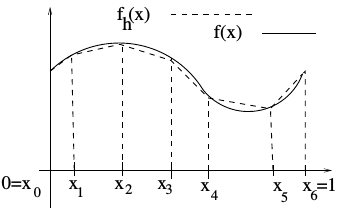
\includegraphics[width=0.4\textwidth]{figure/FEM/polinomilineari}
\caption{Approssimazione $f_{h}$ di una funzione $f(x)$ con polinomi lineari.\label{polinomilineari}}
\end{figure}

L'approssimazione numerica delle equazioni variazionali 
consiste semplicemente nell'approssimazione dello spazio 
delle soluzioni e dello spazio delle funzioni test con spazi finiti dimensionali.
Gli elementi finiti lagrangiani consentono di rappresentare 
la soluzione discretizzata $u_{h}$ sfruttando i valori assunti da $u$ in opportuni punti, chiamati nodi.
Considerando una partizione del dominio $\Omega$ in $N+1$ 
sottointervalli di ampiezza $h_{i}=x_{i+1}-x_{i}$, tali che 
\begin{equation}
\{0= x_{0} < x_{1} < \dots < x_{N}=1 \}\,.
\end{equation}
L'intervallo $[x_{i},x_{i+1}]$ è detto elemento della 
discretizzazione $\Omega_{e}$, mentre i punti $x_{i}$ 
vengono chiamati nodi dell'elemento 
e in corrispondenza di essi vengono definiti i valori
della soluzione discretizzata $u_{h}$. 
Si può associare ad ogni nodo $i$ una numerazione 
locale sull'elemento, ovvero  $x_{1}^{e}=x_{i}, x_{2}^{e}=x_{i+1}$

Il tipo di approssimazione degli spazi, come $L^2(0,1)$ o $H^1(0,1)$, 
determinerà il tipo di metodo usato.
In particolare considerando una approssimazione attraverso polinomi 
lineare lagrangiani è possibile definire una una base dello spazio $X_{h}^{1}$,
contenuta in $H^1(0,1)$, può essere ottenuta dalla combinazione lineare di 
opportune funzioni $\phi^{1}_{i}(x)$, così definite
\begin{equation}
 \phi_{i}^{1}=
 \begin{cases}
  0 & x\leq x_{i-1}\\
  \frac{x-x_{i-1}}{x_{i}-x_{i-1}} & x_{i-1}<x\leq x_{i} \\
  \frac{x_{i+1}-x}{x_{i+1}-x_{i}} & x_{i}\leq x < x_{i+1} \\
  0 & x\geq x_{i+1}\\
 \end{cases}
\,.
\end{equation}
La funzione $\phi_{i}^{1}$ è dunque lineare a tratti ed essa assume il valore $1$ in $x_{i}$ e $0$ 
in tutti gli altri nodi della partizione considerata, approssimando la funzione come 
in figura \ref{polinomilineari}.
Lo spazio dei polinomi lagrangiani lineari dunque risulta
\begin{equation}
 X_{h}^{1}= \{ f \in H^{1}(0,1) : f= \sum_{i=0}^{N}\alpha_{i}\phi_{i}^{1}(x), 
 \alpha_{i} \in \mathbb{R}, \forall i = 0, 1, \dots, N \} \,.
\end{equation}
Data una funzione $u \in H^{1}(0,1)$, è possibile scrivere la 
sua approssimazione $u_{h}$ nello spazio $X_{h}^{1}$
\begin{equation}
 u_{h}=\sum_{i=0}^{N-1} u_{i} \phi_{i}^{1} \quad \forall x \in [0,1]
\end{equation}
dove con $u_{i}$ si è indicato il valore della funzione nel nodo i-esimo $u(x_{i})$.
%%%%%%%%%%%%%%%%%%%%%%%%%%%%%%%%%%%%%%
\begin{figure}[!htb]
\centering
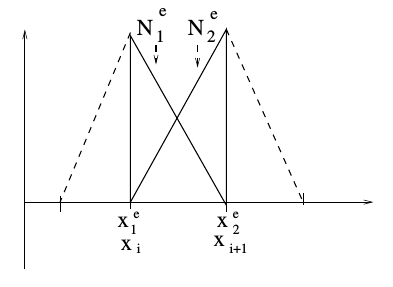
\includegraphics[width=0.4\textwidth]{figure/FEM/funzioniforma}
\caption{\label{funzioniforma} Funzioni di forma Lagrangiane lineari sull'elemento $\Omega_{e}$.}
\end{figure}
%%%%%%%%%%%%%%%%%%%%%%%%%%%%%%%%%%%%%%
In figura \ref{funzioniforma} è evidenziato l'elemento
$\Omega_{e}=[x_{i},x_{i+1}]$ delimitato dai nodi $x^{e}_{1}$ e $x^{e}_{2}$ e indicate
con $N^{1,e}_{1}(x)$ e con $N^{1,e}_{2}(x)$ le restrizioni 
rispettivamente di $\phi_{i}^{1}$ e di $\phi_{i+1}^{1}$ sull'elemento locale $\Omega_{e}$. In ogni
elemento si hanno dunque due funzioni di forma, ciascuna 
delle quali vale $1$ nel punto in cui è definito 
l'indice e $0$ nell'altro. 
Risulta comodo passare ad un sistema di riferimento locale attraverso una 
semplice trasformazione lineare definita
\begin{equation}
 \xi=-1+2\frac{x-x_{i}}{x_{i+1}-x_{i}} \,.
\end{equation}
Le funzioni di forma vengono espresse quindi nell'elemento canonico come segue
\begin{equation}
 N^{1}_{1}(\xi)=
 \begin{cases}
  0 & \xi \leq -1 \\
  \dfrac{1-\xi}{2} & -1 < \xi \geq 1 \\
  0 & \xi > 1 
 \end{cases}
,
\end{equation}
\begin{equation}
 N^{1}_{2}(\xi)=
 \begin{cases}
  0 & \xi \leq -1 \\
  \dfrac{1+\xi}{2} & -1 < \xi \geq 1 \\
  0 & \xi > 1 
 \end{cases}
.
\end{equation}
Se indichiamo con $u_{h}^{e}$ l'approssimazione della
funzione $u$ sull'elemento $\Omega_{e}$ si ottiene la soluzione
discretizzata nello spazio $X^1_h(0,1)$  come
\begin{equation}
 u_{h}^{e}(x)=\sum_{e=1}^{n_{e}}u(x_{i}^{e})N_{i}^{1,e} \quad \text{con} \; x \in [x_{1}^{e},x_{2}^{e}] \, ,
\end{equation}
dove $u(x_{i}^{e})$ è il valore della funzione nel punto $x_{i}^{e}$ dell'elemento. 

\subsection{Discretizzazione dell'equazione di Navier-Stokes}
Si vuole ora descrivere il processo di discretizzazione agli elementi finiti 
applicato all'equazione di Navier-Stokes per una generica geometria e 
condizioni a contorno. 
Consideriamo le equazioni di conservazione della massa e della quantità di moto
per un fluido
\begin{eqnarray}
	 \frac{\partial \rho}{\partial t}+\nabla\cdot (\rho {\bf v})=&& \ 0 \,,\\
	\rho\Big( \frac{\partial {\bf v}}{\partial t}+({\bf v} \cdot \nabla){\bf v} \Big)=
	&&-\nabla p+ \mu \nabla \cdot {\bf \tau}+ \textit{\textbf{f}} \,,
\end{eqnarray}
dove $\rho$ è la densità del fluido, ${\bf v}$ la velocità, ${\bf \tau}$ il tensore degli
sforzi viscosi, $\mu$ la viscosità dinamica, $p$ la pressione e $\textit{\textbf{f}}$ 
un'eventuale forzante al moto. 
Con le dovute assunzioni di fluido newtoniano e incomprimibile ($\rho$ costante)
le equazioni precedenti diventano
\begin{eqnarray} \label{ff2}
	\nabla\cdot  {\bf v}=&&\ 0 \,,\\ 
	\frac{\partial {\bf v}}{\partial t}+({\bf v} \cdot \nabla){\bf v} =
	&& -\frac{\nabla p}{\rho}+ \nu \nabla^{2}{\bf v}+ \textit{\textbf{f}}\,.
\end{eqnarray} 
Si ricorda che tale sistema di equazioni necessita di un adeguato \textit{set} di
condizioni al contorno e di una condizione iniziale per la chiusura, che per ora verranno
omesse per mantenere il caso generale. 

Passiamo alla trasformazione dell'equazione in forma debole.
In primo luogo si considera la derivata temporale, 
discretizzandola come segue (Eulero implicito)
\begin{equation}
\frac{\partial {\bf v}}{\partial t}\cong \frac{{\bf v}-{\bf v}^{old}}{\Delta t}\,.
\end{equation}
La condizione iniziale ci permette di imporre per il primo istante di tempo il valore 
di ${\bf v}^{old}$ come ${\bf v}^{old}={\bf v}(0)$. Passiamo alla forma debole, 
moltiplicando per le funzioni test e integrando 
sul dominio $\Omega$
\begin{eqnarray} 
&& \int_{\Omega} \nabla \cdot {\bf v} \psi dx =0 \,,\\ \label{fdd2} 
&& \int_{\Omega} \frac{ {\bf v}-{\bf v}^{old} }{\Delta t} \cdot {\bf \varphi} dx 
+ \int_{\Omega} (({\bf v} \cdot \nabla){\bf v})\cdot {\bf \varphi} dx=  \nonumber \\ 
&& \qquad \qquad -
\int_{\Omega}\nabla p \cdot {\bf \varphi}dx +\nu \int_{\Omega} \nabla^{2} {\bf v}dx 
+\int_{\Omega} \textbf{f}\cdot {\bf \varphi}dx  \,.
\end{eqnarray}
Le precedenti valgono $\forall  {\bf \varphi}\in \textbf{H}^{1}(\Omega)$ e $\forall  \psi \in L^{2}(\Omega)$. 

Alle equazioni \eqref{fdd2} \`e possibile applicare l'integrazione per parti, 
per eliminare i termini dove è presente la derivata seconda della velocità 
o la derivata prima della pressione per ricavare
\begin{eqnarray} \label{fd33}
	\int_{\Omega} \frac{ {\bf v}-{\bf v}^{old} }{\Delta t} \cdot {\bf \varphi} dx + 
	\int_{\Omega} (({\bf v}^{old} \cdot \nabla){\bf v})\cdot {\bf \varphi} dx &&= \nonumber
	-\int_{\partial\Omega}p \hat{{\bf n}} \cdot {\bf \varphi}ds+\int_{\Omega} p 
	\nabla \cdot {\bf \varphi}dx+ \\  +\nu \int_{\partial \Omega} 
% 	( \vv{\vv{\nabla{\bf v}}}\cdot \hat{{\bf n}}){\bf \varphi} ds- 
	\nu \int_{\Omega} \big( \nabla {\bf v}^{T}{\bf :} 
	\nabla{\bf \varphi} \big) dx +\int_{\Omega} \textbf{f}\cdot
	{\bf \varphi}dx \,,  
\end{eqnarray}
ovviamente ancora valida $\forall  {\bf \varphi}\in \textbf{H}^{1}(\Omega)$. Il termine 
${{\bf v}^{old}}/{\Delta t}$ verr\`a poi inserito nel \textit{Right Hand Side}, 
quindi non farà  parte delle incognite dell'equazione, mentre per risolvere la non linearità 
del termine di avvezione si è sostituito ${\bf v}$ con ${\bf v}^{old}$.
I termini di superficie ricavati dall'integrazione per parti sono intimamente collegati 
alle condizioni al contorno: queste infatti dovranno essere tali da annullare
o definire univocamente il valore di tali integrali sulla superficie, 
affinché il problema risulti ben posto.

Ora si vuole discretizzare l'equazione \eqref{fd33}, 
per permettere il calcolo agli elementi finiti.
Le soluzioni ${\bf v} \ e\  p$ vengono approssimate 
rispettivamente come: ${\bf v}_{h}\in \textbf{X}_{h}^{2}$ e $p_{h}\in X_{h}^{1}$. 
Passiamo quindi alla forma discretizzata e suddividiamo sugli elementi
\begin{flalign} \label{ef1}
\sum_{e=0}^{N_{e}-1} \int_{\Omega_{h}^{e}} \nabla \cdot {\bf v}_{h}^{e}& \psi_{l}^{e} dx =\ 0 \,,  && 
\\ \label{ef22} 
\sum_{e=0}^{N_{e}-1} \bigg[ \int_{\Omega_{h}^{e}} \frac{ 
{\bf v}_{h}^{e} }{\Delta t} \cdot &{\bf \varphi}_{i}^{e} dx  + 
\int_{\Omega_{h}^{e}} (({\bf v}_{h}^{e} \cdot \nabla){\bf v}_{h}^{e})\cdot 
{\bf \varphi}_{i}^{e} dx \bigg] = \\&
\sum_{e=0}^{N_{e}-1} 
\bigg[ \int_{\Omega} p_{h} \nabla \cdot {\bf \varphi}_{i}^{e}dx + 
- \nu \int_{\Omega_{h}^{e}} \big({\nabla {\bf v}_{h}^{e}}^{T}{\bf :} 
\nabla{\bf \varphi}_{i}^{e} \big) dx +
\int_{\Omega_{h}^{e}} \textbf{f}\cdot {\bf \varphi}_{i}^{e}dx \bigg]  \,.\nonumber
\end{flalign}
Le precedenti valgono rispettivamente
 $\forall \psi_{l}^{e} \in X_{h}^{1}$  con  $l=0,...,N_{p}-1 $ e 
 $\forall {\bf \varphi}_{i}^{e} \in \textbf{X}_{h}^{2}$ con $i=0,...,N_{v}-1$,
 dove $N_{p}$ e $N_v$ sono rispettivamente il numero dei nodi totali nel caso di 
discretizzazione lineare e quadratica. Nella trattazione seguente verranno rimossi 
i termini di superficie per alleggerire l'esposizione,
i quali verranno calcolati una volta note le condizioni a contorno. 
Ricordando il valore delle seguenti
\begin{equation}\renewcommand{\arraystretch}{1.6}\setlength{\arraycolsep}{5pt}
 {\bf v}_{h}^{e}=\sum_{j=1}^{n_v} {\bf v}_{j}^{e}N_{j}^{(2,e)}\,,
\end{equation} 
\begin{equation}
p_{h}^{e}=\sum_{j=1}^{n_p} p_{j}^{e}N_{j}^{(1,e)}\,,
\end{equation}
si ricava dalle \eqref{ef1} e \eqref{ef22}
\begin{equation} \label{ef11}
\sum_{j=1}^{n_p} \sum_{e=0}^{N_{e}-1} \int_{\Omega_{h}^{e}} \nabla 
\cdot ({\bf v}_{j}^{e}N_{j}^{(2,e)}) \psi_{l}^{e} dx=0 \,,
\end{equation}
\vspace{-5mm}
\begin{flalign} \label{ef222} 
\sum_{j=1}^{n_v} \sum_{e=0}^{N_{e}-1} \bigg[ \int_{\Omega_{h}^{e}} 
\frac{ {\bf v}_{j}^{e}N_{j}^{(2,e)} }{\Delta t}  
\cdot {\bf \varphi}_{i}^{e} dx + &\int_{\Omega_{h}^{e}} 
((({\bf v}_{j}^{e}N_{j}^{(2,e)}) \cdot \nabla)({\bf v}_{j}^{e}N_{j}^{(2,e)}))
\cdot {\bf \varphi}_{i}^{e} dx \bigg] = \nonumber
\\ =\sum_{j=1}^{n_v} 
\sum_{e=0}^{N_{e}-1} \bigg[ -\sum_{k=1}^{4} &\int_{\Omega_{h}^{e}}
(p_{k}^{e}N_{k}^{(1,e)}) \nabla \cdot {\bf \varphi}_{i}^{e} dx -
\\ -\nu & \int_{\Omega_{h}^{e}} \big(\nabla \big(({\bf v}_{j}^{e}N_{j}^{(2,e)})\big)^{T}{\bf :}
\nabla{\bf \varphi}_{i}^{e} \big) dx +\int_{\Omega_{h}^{e}} \textbf{f}
\cdot {\bf \varphi}_{i}^{e}dx \bigg] \,.  \nonumber
\end{flalign}
Considerando un generico elemento, le precedenti equazioni valgono per ogni funzione test non 
nulla sull'elemento considerato, dove $n_v$ e $n_p$ sono il numero di nodi per il singolo elemento, 
quindi per un caso tridimensionale con elementi HEX27 le due precedenti rappresentano 
in realtà un \textit{set} di 89 equazioni (27 per le $\varphi_{u}$, 
27 per le $\varphi_{v}$, 27 per le $\varphi_w$ e 8 per le $\psi$), ricordando che le variazioni 
sono indipendenti, e quindi le equazioni per le $u$ si ricavano ponendo $\varphi_{v}=0$ 
e $\varphi_w=0$, e viceversa. 

Al fine di ridurre il problema ad un sistema algebrico, si vuole trasformare l'elemento $\Omega_e$
nell'elemento canonico $\hat{\Omega}$ utilizzando l'ormai nota trasformazione
\begin{equation}
	x^e(\xi,\eta,\zeta)=\sum_{j=1}^{n_v}x_j^e N_j^{(2,e)}(\xi,\eta,\zeta) \,,
\end{equation}
il cui Jacobiano vale
{
	\everymath{\displaystyle}
\begin{equation}\renewcommand{\arraystretch}{1.6}\setlength{\arraycolsep}{4pt}
	\mathcal{J}=\begin{bmatrix}
\sum_{j=1}^{n_v}x_j^e\frac{\partial N_j^{(2,e)}}{\partial \xi} &
\sum_{j=1}^{n_v}x_j^e\frac{\partial N_j^{(2,e)}}{\partial \eta} &
\sum_{j=1}^{n_v}x_j^e\frac{\partial N_j^{(2,e)}}{\partial \zeta}\\
\sum_{j=1}^{n_v}y_j^e\frac{\partial N_j^{(2,e)}}{\partial \xi} &
\sum_{j=1}^{n_v}y_j^e\frac{\partial N_j^{(2,e)}}{\partial \eta} &
\sum_{j=1}^{n_v}y_j^e\frac{\partial N_j^{(2,e)}}{\partial \zeta} \\
\sum_{j=1}^{n_v}z_j^e\frac{\partial N_j^{(2,e)}}{\partial \xi} &
\sum_{j=1}^{n_v}z_j^e\frac{\partial N_j^{(2,e)}}{\partial \eta} &
\sum_{j=1}^{n_v}z_j^e\frac{\partial N_j^{(2,e)}}{\partial \zeta} &
\end{bmatrix}_{(\xi,\eta,\zeta)}
\end{equation}
}%
Per il cambiamento di variabile da globale a canonico è necessaria l'inversa
dello $\mathcal{J}$, che può essere facilmente ricavato con note tecniche
algebriche
\begin{eqnarray}\renewcommand{\arraystretch}{1.4}\setlength{\arraycolsep}{5pt}
	\mathcal{J}^{-1}=
 \begin{bmatrix}
\frac{\displaystyle\partial \xi}{\displaystyle\partial x} &
\frac{\displaystyle\partial \xi}{\displaystyle\partial y} & 
\frac{\displaystyle\partial \xi}{\displaystyle\partial z} \\
\frac{\displaystyle\partial \eta}{\displaystyle\partial x} &
\frac{\displaystyle\partial \eta}{\displaystyle\partial y}&
\frac{\displaystyle\partial \eta}{\displaystyle\partial z} \\
\frac{\displaystyle\partial \zeta}{\displaystyle\partial x} &
\frac{\displaystyle\partial \zeta}{\displaystyle\partial y}& 
\frac{\displaystyle\partial \zeta}{\displaystyle\partial z}
\end{bmatrix}_{(\xi,\eta,\zeta)}
\end{eqnarray}
Con le precedenti infatti è possibile calcolare le derivate di una generica funzione come
\begin{equation}
\begin{split}
	& \frac{\partial f_h}{\partial x}({\bf x^e})=\frac{\partial \xi}{\partial x}\frac{d f_h}{d \xi}
+\frac{\partial \eta}{\partial x}\frac{d f_h}{d \eta}
+\frac{\partial \zeta}{\partial x}\frac{d f_h}{d \zeta}= \\
	& \quad \quad \sum_{j=1}^{n_v} f_j^e({\bf x_j^e}) \left(
\frac{\partial \xi}{\partial x}\frac{d N_j^{(2,e)}}{d \xi}+
\frac{\partial \eta}{\partial x}\frac{d N_j^{(2,e)}}{d \eta}
\frac{\partial \zeta}{\partial x}\frac{d N_j^{(2,e)}}{d \zeta}
\right)
\end{split}\,.
\end{equation}
L'equazione \eqref{ef222} può essere rappresentata in forma compatta per un singolo elemento come
\begin{equation}
\mathcal{A}_{h}^{e}{\bf \chi}_{h}^{e}=\textbf{b}_{h}^{e}\,,
\end{equation}
dove le precedenti possono essere rappresentate dalle seguenti
sottomatrici 
e sottovettori
\begin{eqnarray}\renewcommand{\arraystretch}{1.5}\setlength{\arraycolsep}{5pt}
\mathcal{A}_h^e=
\begin{bmatrix}
\textbf{D}_h^e & \textbf{B}_h^e\\
(\textbf{B}_h^e)^T & 0
\end{bmatrix} \qquad
{\bf \chi}_h^e= \begin{bmatrix}
{\bf v}_h^e \\
 p_h^e
\end{bmatrix} \qquad
\textbf{b}_h^e= \begin{bmatrix}
\textbf{f}_h^{\,e} \\
 0
\end{bmatrix}\,.
\end{eqnarray}
Più nello specifico, le matrici \textbf{D}$_h^e$ e \textbf{B}$_h^e$ sono composte dalle seguenti
ulteriori sottomatrici (si sta considerando il generico caso tridimensionale)
\begin{eqnarray}\renewcommand{\arraystretch}{1.5}\setlength{\arraycolsep}{4pt}
\textbf{ D}_h^e= \begin{bmatrix}
\textbf{D}_{h,1}^e & 0 & 0\\
0 & \textbf{D}_{h,2}^e & 0\\
0 & 0 & \textbf{D}_{h,3}^e
\end{bmatrix} \qquad
\textbf{B}_h^e=
\begin{bmatrix}
\textbf{B}_{h,1}^e \\
 \textbf{B}_{h,2}^e \\
 \textbf{B}_{h,3}^e
\end{bmatrix}\,.
\end{eqnarray}
Ciascuna matrice \textbf{D}$_{h,k}^e$ è simmetrica, formata da $n_v \times n_v$ elementi.
Si può rappresentare il generico elemento della $k$-esima matrice \textbf{D}$_{h,k}^e$ come
\begin{eqnarray}
(D_{h,k}^e)_{i,j}=\int_{\Omega_e}\frac{N_j^{(2,e)}}{\Delta t}\cdot N_i^{(2,e)}\ d \Omega
	+\int_{\Omega_e}[({\bf v}^{old}
	\cdot\nabla) N_j^{(2,e)}]N_i^{(2,e)} \ d\Omega
 + \\
	+  \nu\int_{\Omega_e} (\nabla N_j^{(2,e)}:\nabla N_i^{(2,e)}) \ d\Omega \,.
 \nonumber
\end{eqnarray}
Ogni matrice \textbf{B}$_{h,k}^e$ è formata da $n_{v} \times n_{p}$ elementi
che possono esprimersi come
\begin{equation}
	(B_{h,k}^e)_{i,j}=\int_{\Omega_e}N_i^{(1,e)}\frac{\partial}{\partial x_{k}} N_j^{(2,e)} \ d\Omega\,. 
\end{equation}
La matrice \textbf{B}$_h^e$ tiene conto del termine relativo 
al gradiente di pressione nell'equazione di conservazione della
quantità di moto, mentre la sua trasposta, ovvero le "righe" della
matrice $\mathcal{A}_h^e$ relative ai termini di pressione,
deriva dall'equazione di continuità.

Il vettore del \textit{right hand side} \textbf{f}$_h^e$ è composto da $3n_v$ elementi
che possono essere espressi come
\begin{equation}
	(f_{h,k}^e)_i=\int_{\Omega_e}f_k^e N_i^{(2,e)} \ d\Omega \,.
\end{equation}
Passaggio fondamentale è quello di inserire gli elementi della matrice
locale $\mathcal{A}_h^e$ all'interno della matrice globale; per fare ciò 
è necessaria una mappa della connettività, che lega ciascun elemento locale 
con il corrispettivo globale.

Un piccolo inciso sulle condizioni a contorno: affinché vengano applicate correttamente 
è necessario, come già detto, che i contributi di superficie siano ben definiti, o nulli.
Nell'applicazione delle condizioni a contorno quindi, nel caso di condizioni di
Neumann, gli integrali di superficie vengono calcolati con il valore di \textit{boundary}
e inseriti nel \textit{right hand side} dell'equazione.
Per il caso di condizioni di Dirichlet più semplicemente
vengono annullate le righe relative ai nodi appartenenti al bordo, fatta eccezione 
per i valori sulla diagonale che vengono posti uguali ad uno, e il valore della condizione
a contorno viene quindi imposta in modo forzato
nel \textit{right hand side} relativo ai nodi in questione.


 







